% Options for packages loaded elsewhere
\PassOptionsToPackage{unicode}{hyperref}
\PassOptionsToPackage{hyphens}{url}
%
\documentclass[
]{article}
\usepackage{lmodern}
\usepackage{amssymb,amsmath}
\usepackage{ifxetex,ifluatex}
\ifnum 0\ifxetex 1\fi\ifluatex 1\fi=0 % if pdftex
  \usepackage[T1]{fontenc}
  \usepackage[utf8]{inputenc}
  \usepackage{textcomp} % provide euro and other symbols
\else % if luatex or xetex
  \usepackage{unicode-math}
  \defaultfontfeatures{Scale=MatchLowercase}
  \defaultfontfeatures[\rmfamily]{Ligatures=TeX,Scale=1}
  \setmainfont[]{texgyrepagella-regular.otf}
  \setsansfont[]{Fira Sans}
\fi
% Use upquote if available, for straight quotes in verbatim environments
\IfFileExists{upquote.sty}{\usepackage{upquote}}{}
\IfFileExists{microtype.sty}{% use microtype if available
  \usepackage[]{microtype}
  \UseMicrotypeSet[protrusion]{basicmath} % disable protrusion for tt fonts
}{}
\makeatletter
\@ifundefined{KOMAClassName}{% if non-KOMA class
  \IfFileExists{parskip.sty}{%
    \usepackage{parskip}
  }{% else
    \setlength{\parindent}{0pt}
    \setlength{\parskip}{6pt plus 2pt minus 1pt}}
}{% if KOMA class
  \KOMAoptions{parskip=half}}
\makeatother
\usepackage{xcolor}
\IfFileExists{xurl.sty}{\usepackage{xurl}}{} % add URL line breaks if available
\IfFileExists{bookmark.sty}{\usepackage{bookmark}}{\usepackage{hyperref}}
\hypersetup{
  pdftitle={Supplementary Material},
  pdfauthor={Grant McDermott},
  hidelinks,
  pdfcreator={LaTeX via pandoc}}
\urlstyle{same} % disable monospaced font for URLs
\usepackage[margin=1in]{geometry}
\usepackage{graphicx}
\makeatletter
\def\maxwidth{\ifdim\Gin@nat@width>\linewidth\linewidth\else\Gin@nat@width\fi}
\def\maxheight{\ifdim\Gin@nat@height>\textheight\textheight\else\Gin@nat@height\fi}
\makeatother
% Scale images if necessary, so that they will not overflow the page
% margins by default, and it is still possible to overwrite the defaults
% using explicit options in \includegraphics[width, height, ...]{}
\setkeys{Gin}{width=\maxwidth,height=\maxheight,keepaspectratio}
% Set default figure placement to htbp
\makeatletter
\def\fps@figure{htbp}
\makeatother
\setlength{\emergencystretch}{3em} % prevent overfull lines
\providecommand{\tightlist}{%
  \setlength{\itemsep}{0pt}\setlength{\parskip}{0pt}}
\setcounter{secnumdepth}{-\maxdimen} % remove section numbering
\usepackage{fontspec}
\usepackage{booktabs}
\usepackage{tabularx}
\usepackage{threeparttable}
\usepackage{dcolumn}
\newcolumntype{A}{D{.}{.}{2.3}}
\usepackage{sectsty} % Allows your to change titles style
\allsectionsfont{\sffamily} % Define the style of all titles
\usepackage{booktabs}
\usepackage{longtable}
\usepackage{array}
\usepackage{multirow}
\usepackage{wrapfig}
\usepackage{float}
\usepackage{colortbl}
\usepackage{pdflscape}
\usepackage{tabu}
\usepackage{threeparttable}
\usepackage{threeparttablex}
\usepackage[normalem]{ulem}
\usepackage{makecell}
\usepackage{xcolor}
\ifluatex
  \usepackage{selnolig}  % disable illegal ligatures
\fi
\usepackage[]{natbib}
\bibliographystyle{plainnat}

\title{Supplementary Material}
\usepackage{etoolbox}
\makeatletter
\providecommand{\subtitle}[1]{% add subtitle to \maketitle
  \apptocmd{\@title}{\par {\large #1 \par}}{}{}
}
\makeatother
\subtitle{Sceptic priors and climate consensus}
\author{Grant McDermott}
\date{}

\begin{document}
\maketitle

\newcommand{\beginsupplement}{%
    \setcounter{table}{0}
    \renewcommand{\thetable}{SM\arabic{table}}%
    \setcounter{figure}{0}
    \renewcommand{\thefigure}{SM\arabic{figure}}%
}
%
    \setcounter{table}{0}
    \renewcommand{\thetable}{SM\arabic{table}}%
    \setcounter{figure}{0}
    \renewcommand{\thefigure}{SM\arabic{figure}}%

\listoftables
\listoffigures
\newpage

\hypertarget{tables}{%
\section{Tables}\label{tables}}

\hypertarget{sensitivity-analysis}{%
\subsection{Sensitivity analysis}\label{sensitivity-analysis}}

\begin{table}[ht] \centering 
    \caption{TCR efficacies used in ``MEA'' I and II sensitivity runs} 
    \label{tab:marvel} 
    \begin{threeparttable} 
        \begin{tabularx}{.75\textwidth}{@{\extracolsep{5pt}} Xcc}
            \toprule
            Forcing agent & Mean &   95\% C.I.   \\ 
            \midrule
            Aerosols      & 1.55 & (1.05, 2.05)  \\
            GHGs          & 1.17 & (1.07, 1.28)  \\
            Land use      & 3.82 & (-2.16, 9.80) \\
            Ozone         & 0.66 & (0.34, 0.98)  \\
            Solar         & 1.68 & (-1.27, 4.63)  \\
            Volcanic      & 0.61 & (0.33, 0.89)  \\ 
            \bottomrule
        \end{tabularx} 
        \begin{tablenotes}
            \footnotesize
            \item Notes: Adapted from Table S1 of \cite{marvel2016implications}. Confidence intervals on the sample means are constructed from a \textit{t} distribution with 4 degrees of freedom.
        \end{tablenotes}
    \end{threeparttable} 
\end{table}

\hypertarget{future-temperatures}{%
\subsection{Future temperatures}\label{future-temperatures}}

\begin{table}[h] \centering 
    \caption{Covariate vectors for 2100 predictions} 
    \begin{threeparttable} %%% added %%% 
        \begin{tabularx}{.75\textwidth}{@{\extracolsep{1pt}} X A A A A } 
            %\begin{tabularx}{\textwidth}{X c c c c} 
            %\hline\hline
            \toprule
            &\multicolumn{1}{c}{RCP 2.6}&\multicolumn{1}{c}{RCP 4.5}&\multicolumn{1}{c}{RCP 6.0}&\multicolumn{1}{c}{RCP 8.5}\\
            %&\multicolumn{1}{c}{\footnotesize420 ppmv CO$_2$}&\multicolumn{1}{c}{\footnotesize540 ppmv CO$_2$}&\multicolumn{1}{c}{\footnotesize670 ppmv CO$_2$}&\multicolumn{1}{c}{\footnotesize940 ppmv CO$_2$}\\
            %\hline
            %\\[-1.8ex] 
            \midrule
            $RF_{2100}$                                                                             & 2.626     & 4.281     & 5.522     & 8.340     \\ 
            \hspace{5 pt} \textit{CO$_2$ component} & \multicolumn{1}{c}{\textit{\hspace{1em}85\%}} &   \multicolumn{1}{c}{\textit{\hspace{1em}83\%}}   &   \multicolumn{1}{c}{\textit{\hspace{1em}86\%}}   &   \multicolumn{1}{c}{\textit{\hspace{1em}78\%}}   \\
            \hspace{5 pt} \textit{Solar component}      & \multicolumn{1}{c}{\textit{\hspace{1em} 7\%}} &   \multicolumn{1}{c}{\textit{\hspace{1em} 4\%}}   &   \multicolumn{1}{c}{\textit{\hspace{1em} 3\%}}   &   \multicolumn{1}{c}{\textit{\hspace{1em} 2\%}}   \\
            \\[-1.8ex] 
            $\overline{VOLC}$                                                                   & 0.017     & 0.017     & 0.017     & 0.017     \\
            \\[-1.8ex] 
            $\overline{SOI}$                                                                    &\text{-}0.079  &\text{-}0.079  &\text{-}0.079  &\text{-}0.079  \\
            \\[-1.8ex] 
            $\overline{AMO}$                                                                    &\text{-}0.002 &\text{-}0.002   &\text{-}0.002  &\text{-}0.002  \\
            %\hline\hline
            \bottomrule
        \end{tabularx}
        \begin{tablenotes}
            \footnotesize
            \item \textit{Notes:} Covariates are used to predict the global mean surface temperature anomaly in the year 2100. The Representative Concentration Pathways (RCPs) are a family of forcing scenarios developed for the IPCC \cite{van2011rcp}. Each RCP has a core component of atmospheric CO$_2$ concentrations, measured in parts per million volume (ppmv). With regard to the covariates in the regression model, total radiative forcing ($RF$) and volcanic aerosols ($VOLC$) are measured in Wm$^{-2}$. The Southern Oscillation Index ($SOI$) and Atlantic Multidecadal Oscilliation ($AMO$) are measured as scaled indices. Future values for $RF$ are taken from the RCP database. For the rest, historical mean values are used.
        \end{tablenotes}
    \end{threeparttable} 
    \label{tab:covariate}
\end{table}

\newpage
\pagebreak

\hypertarget{figures}{%
\section{Figures}\label{figures}}

\hypertarget{sensitivity-analysis-1}{%
\subsection{Sensitivity analysis}\label{sensitivity-analysis-1}}

Figs. \ref{fig:sens_cw14} -- \ref{fig:sens_co2} provide additional
context and information related to the various sensitivity analyses
undertaken in Section 5.2 of the main text. In each case, the figure
caption references against the key listed in first column of Table 4.
The figures themselves are directly comparable with Fig. 1 and the same
general notes apply (dashed lines denote TCR priors, solid lines denote
TCR posteriors, etc.) Note that in some cases the x-axis has been
truncated to preserve this direct comparability, even though the
posterior distributions may extend beyond the -1 °C to 3 °C range.

\begin{figure}

{\centering 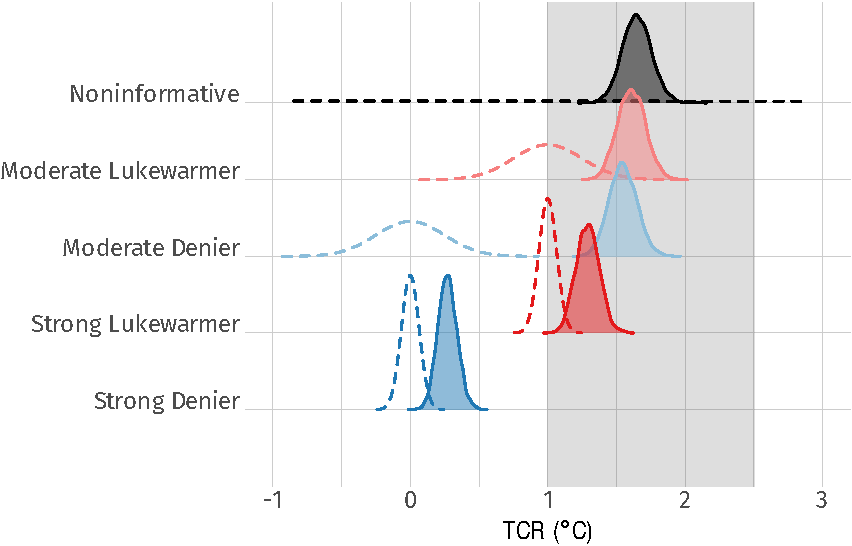
\includegraphics[width=1\linewidth]{/home/grant/Documents/Papers/Sceptic/sceptic-priors/figs/sens_cw14-1} 

}

\caption{TCR densities: "CW14" sensitivity run.}\label{fig:sens_cw14}
\end{figure}

\begin{figure}

{\centering 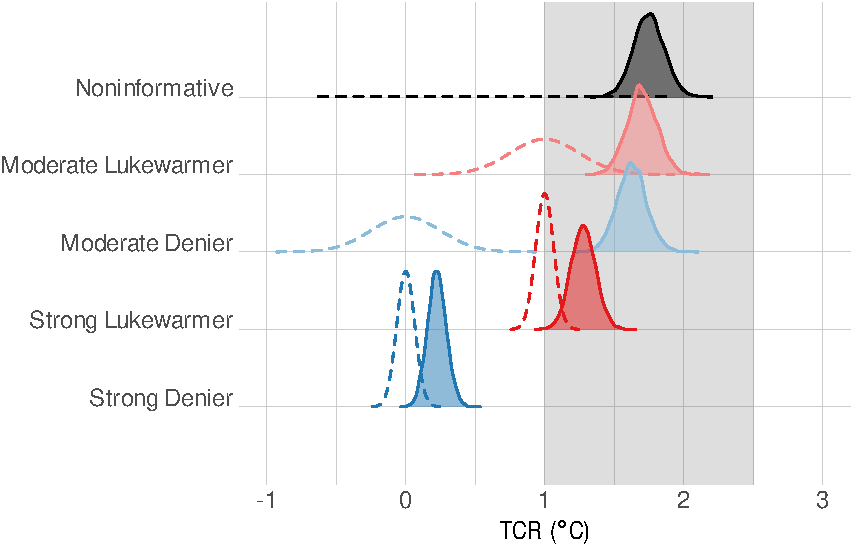
\includegraphics[width=1\linewidth]{/home/grant/Documents/Papers/Sceptic/sceptic-priors/figs/sens_gistemp-1} 

}

\caption{TCR densities: "GISTEMP" sensitivity run.}\label{fig:sens_gistemp}
\end{figure}

\begin{figure}

{\centering 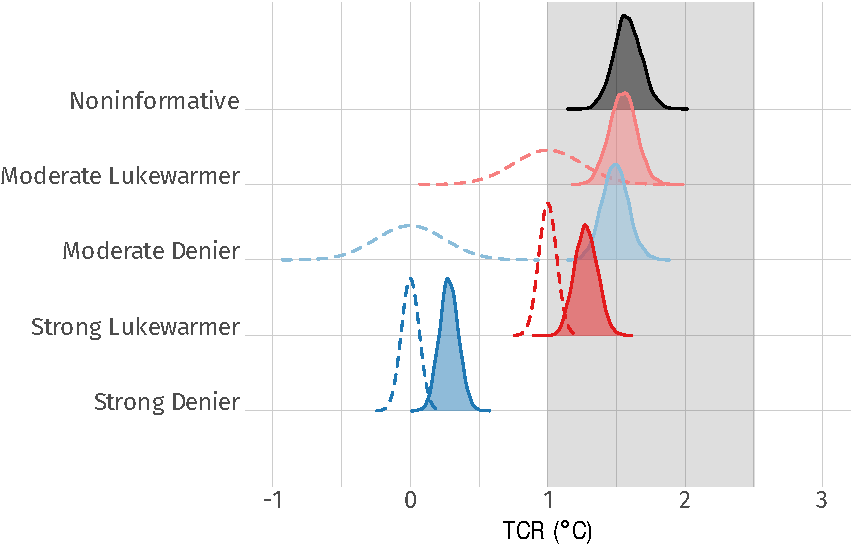
\includegraphics[width=1\linewidth]{/home/grant/Documents/Papers/Sceptic/sceptic-priors/figs/sens_hadcrut_me-1} 

}

\caption{TCR densities: "HadCRUT ME" sensitivity run.}\label{fig:sens_hadcrut_me}
\end{figure}

\begin{figure}

{\centering 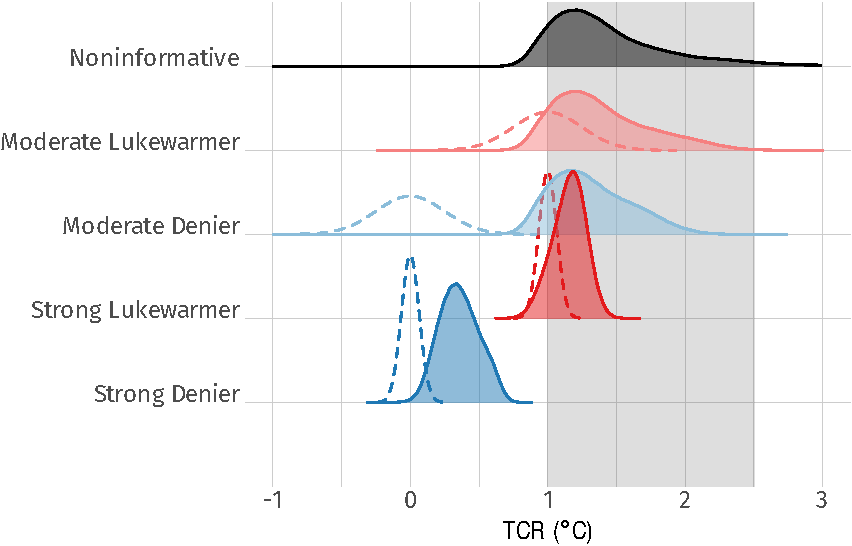
\includegraphics[width=1\linewidth]{/home/grant/Documents/Papers/Sceptic/sceptic-priors/figs/sens_df18-1} 

}

\caption{TCR densities: "DF18" sensitivity run.}\label{fig:sens_df18}
\end{figure}

\begin{figure}

{\centering 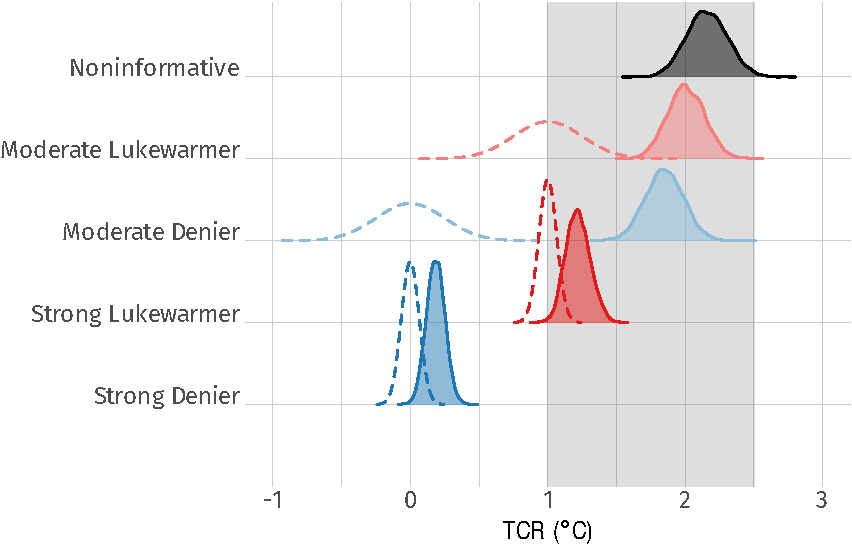
\includegraphics[width=1\linewidth]{/home/grant/Documents/Papers/Sceptic/sceptic-priors/figs/sens_mea_i-1} 

}

\caption{TCR densities: "MEA I" sensitivity run.}\label{fig:sens_mea_i}
\end{figure}

\begin{figure}

{\centering 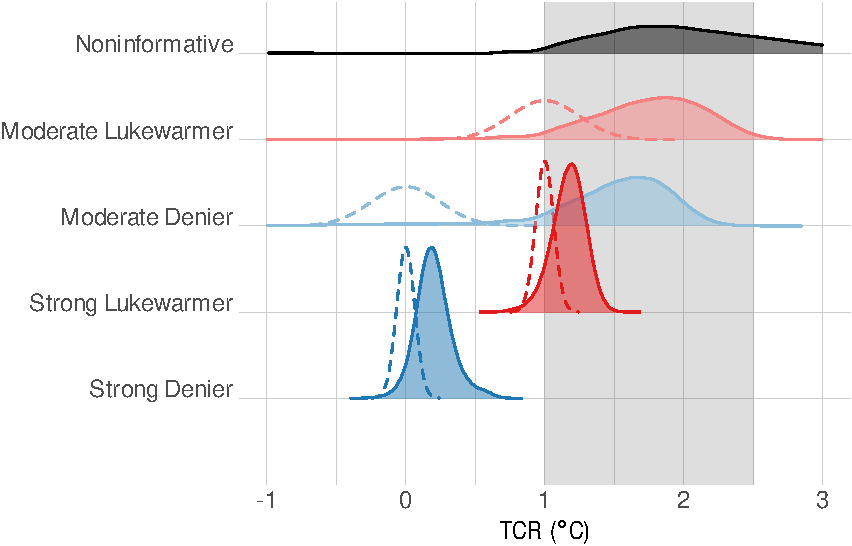
\includegraphics[width=1\linewidth]{/home/grant/Documents/Papers/Sceptic/sceptic-priors/figs/sens_mea_ii-1} 

}

\caption{TCR densities: "MEA II" sensitivity run.}\label{fig:sens_mea_ii}
\end{figure}

\begin{figure}

{\centering 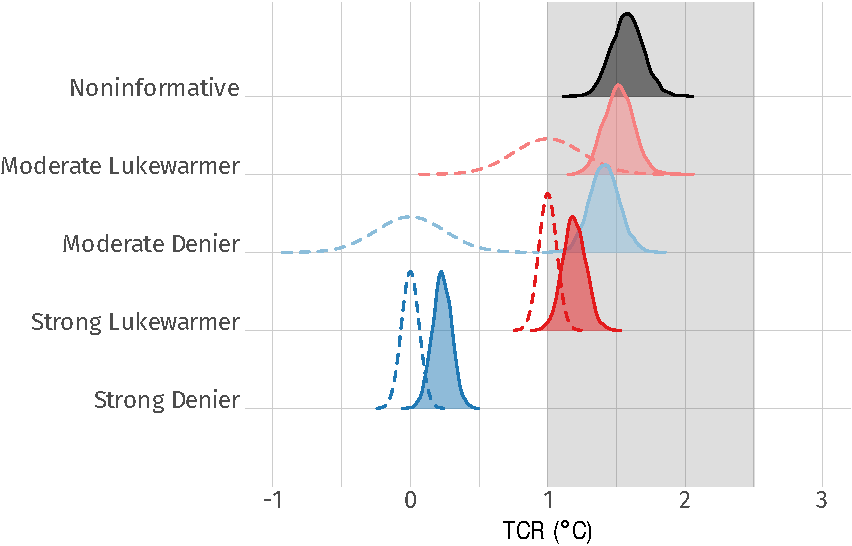
\includegraphics[width=1\linewidth]{/home/grant/Documents/Papers/Sceptic/sceptic-priors/figs/sens_anthro-1} 

}

\caption{TCR densities: "Anthro" sensitivity run.}\label{fig:sens_anthro}
\end{figure}

\begin{figure}

{\centering 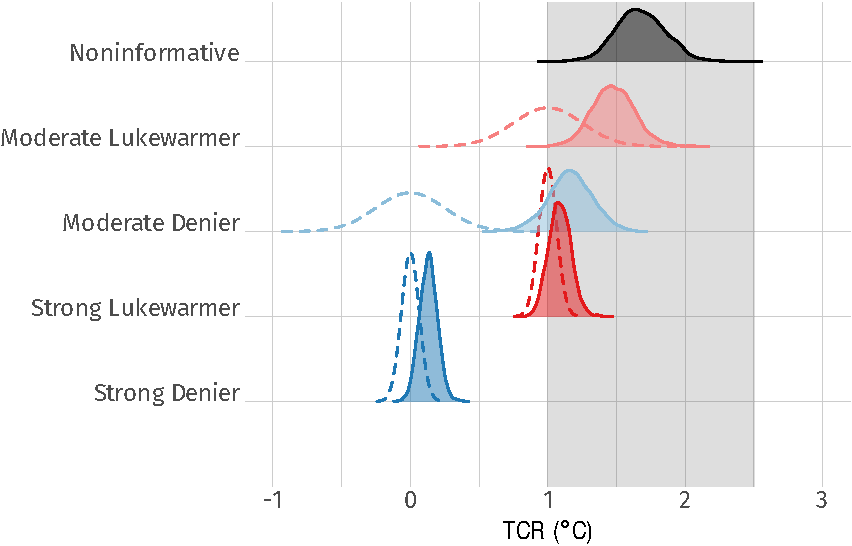
\includegraphics[width=1\linewidth]{/home/grant/Documents/Papers/Sceptic/sceptic-priors/figs/sens_co2-1} 

}

\caption{TCR densities: "CO2" sensitivity run.}\label{fig:sens_co2}
\end{figure}

\pagebreak

\hypertarget{welfare-implications-and-the-social-cost-of-carbon}{%
\subsection{Welfare implications and the social cost of
carbon}\label{welfare-implications-and-the-social-cost-of-carbon}}

\begin{figure}[h]

{\centering 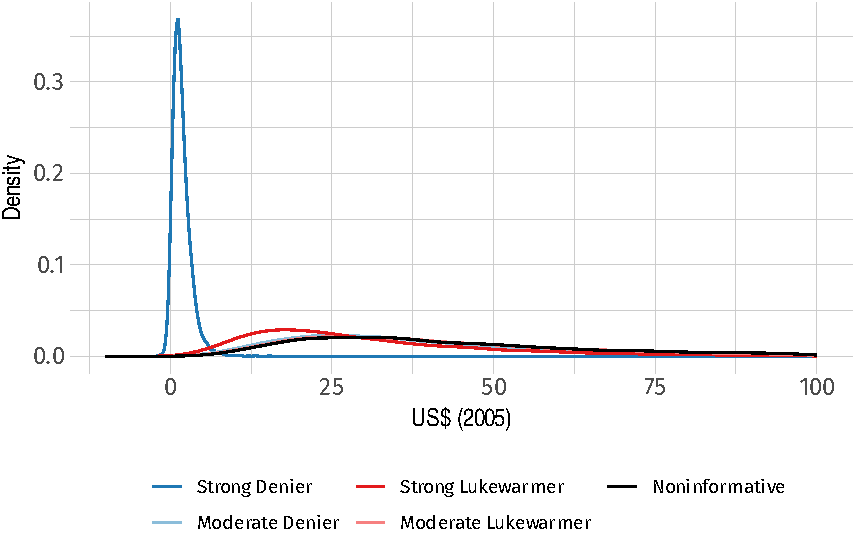
\includegraphics[width=1\linewidth]{/home/grant/Documents/Papers/Sceptic/sceptic-priors/figs/scc-fig-1} 

}

\caption{Social cost of carbon (US\$2005 per ton). The results for each agent type are obtained from 10,000 simulation runs of PAGE \cite{hope2011page09}. Posterior TCR distributions serve as key inputs to the model, while the remaining parameters are set to the PAGE model defaults. The x-axis is truncated at 100 to aid visual inspection; the uppermost tails of the distributions being well in excess of the range given here.}\label{fig:scc-fig}
\end{figure}

\newpage

  \bibliography{../sceptic/sceptic.bib}

\end{document}
